\section{Phân tích khám phá dữ liệu}
Biểu đồ về phân bố dữ liệu theo số ký tự, với giới hạn của số ký tự trong dataset là $(0,5000]$. Đối với tiếng Việt hoặc tiếng Anh, nhóm thấy việc chuẩn hóa theo dạng NFC\footnote{\url{https://unicode.org/reports/tr15/\#Norm\_Forms}} rồi tách từ là đủ, không cần sử dụng đến grapheme cluster\footnote{\url{https://www.unicode.org/reports/tr29/\#Grapheme\_Cluster\_Boundaries}}.

Biểu đồ phân bố dữ liệu theo số từ được tạo ra bằng cách dùng hàm word\_tokenize\footnote{\url{https://www.nltk.org/api/nltk.tokenize.html}} của thư viện NLTK, sau đó bỏ đi các dấu câu.
\begin{figure}[htb]
    \centering
    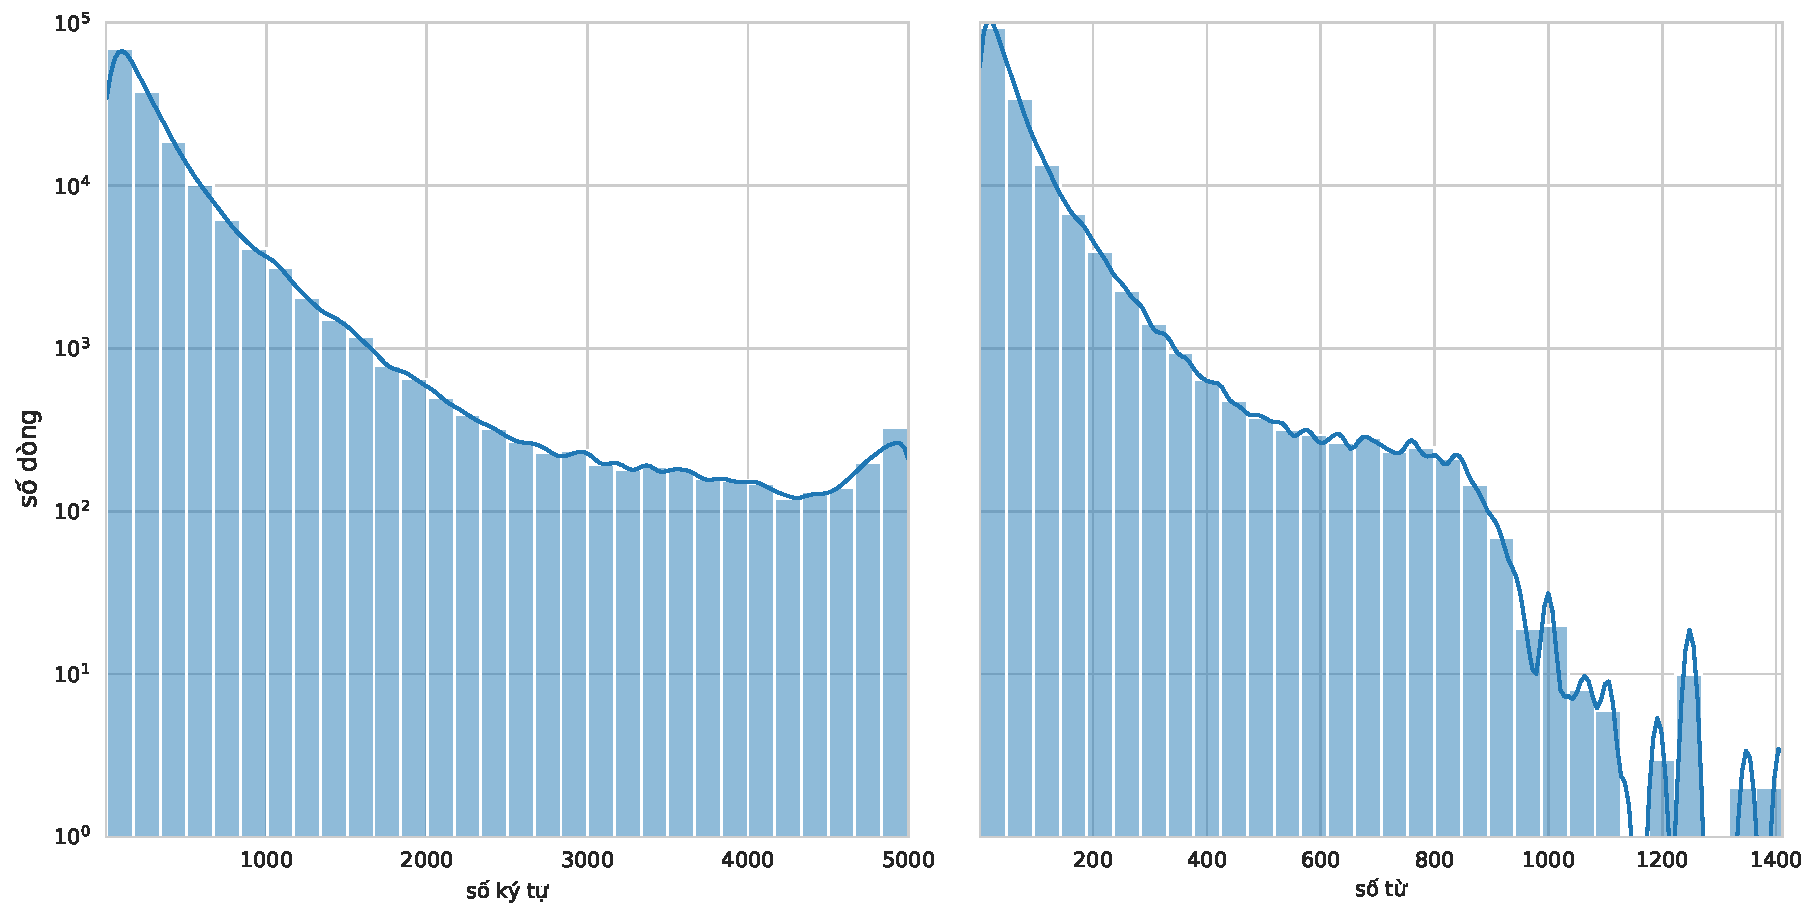
\includegraphics[width=0.9\textwidth]{chapter_2/image/dist_num_chars_and_words.pdf}
    \caption{Phân bố dữ liệu theo số ký tự và theo số từ}
    \label{figure:dist_num_chars_and_words}
\end{figure}
\begin{figure}[htb]
    \centering
    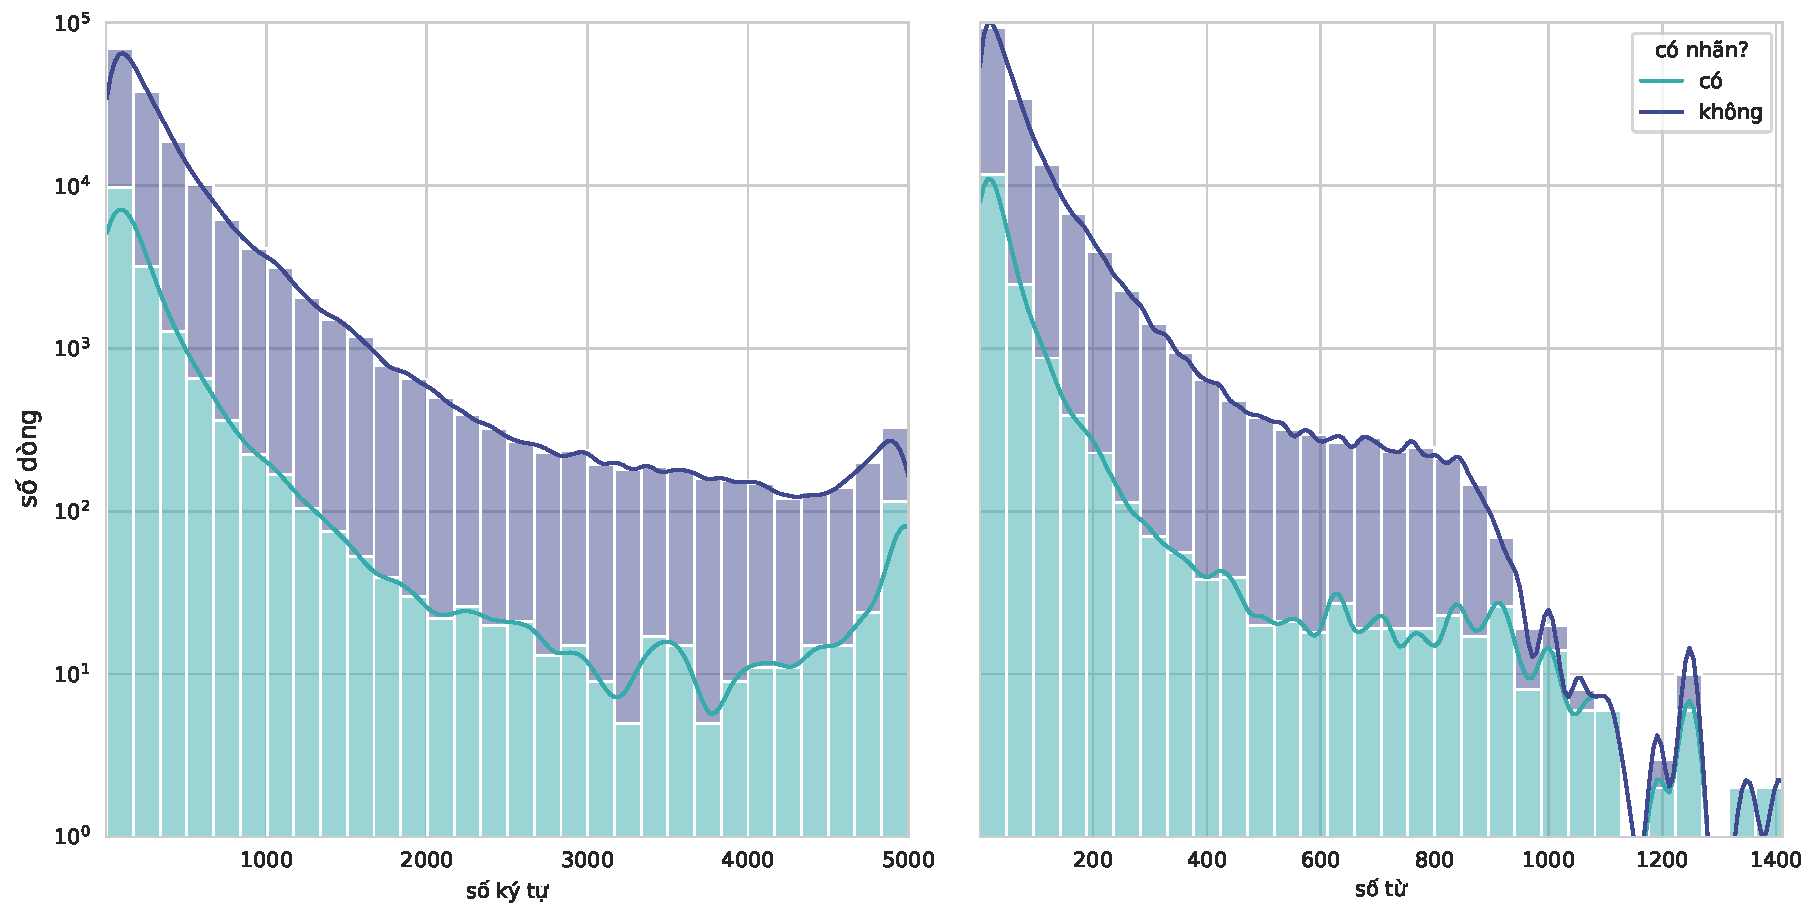
\includegraphics[width=0.9\textwidth]{chapter_2/image/dist_num_chars_and_words_by_has_label.pdf}
    \caption{Phân bố dữ liệu có/không có nhãn theo số ký tự và số từ}
\end{figure}

\begin{figure}[htb]
    \centering
    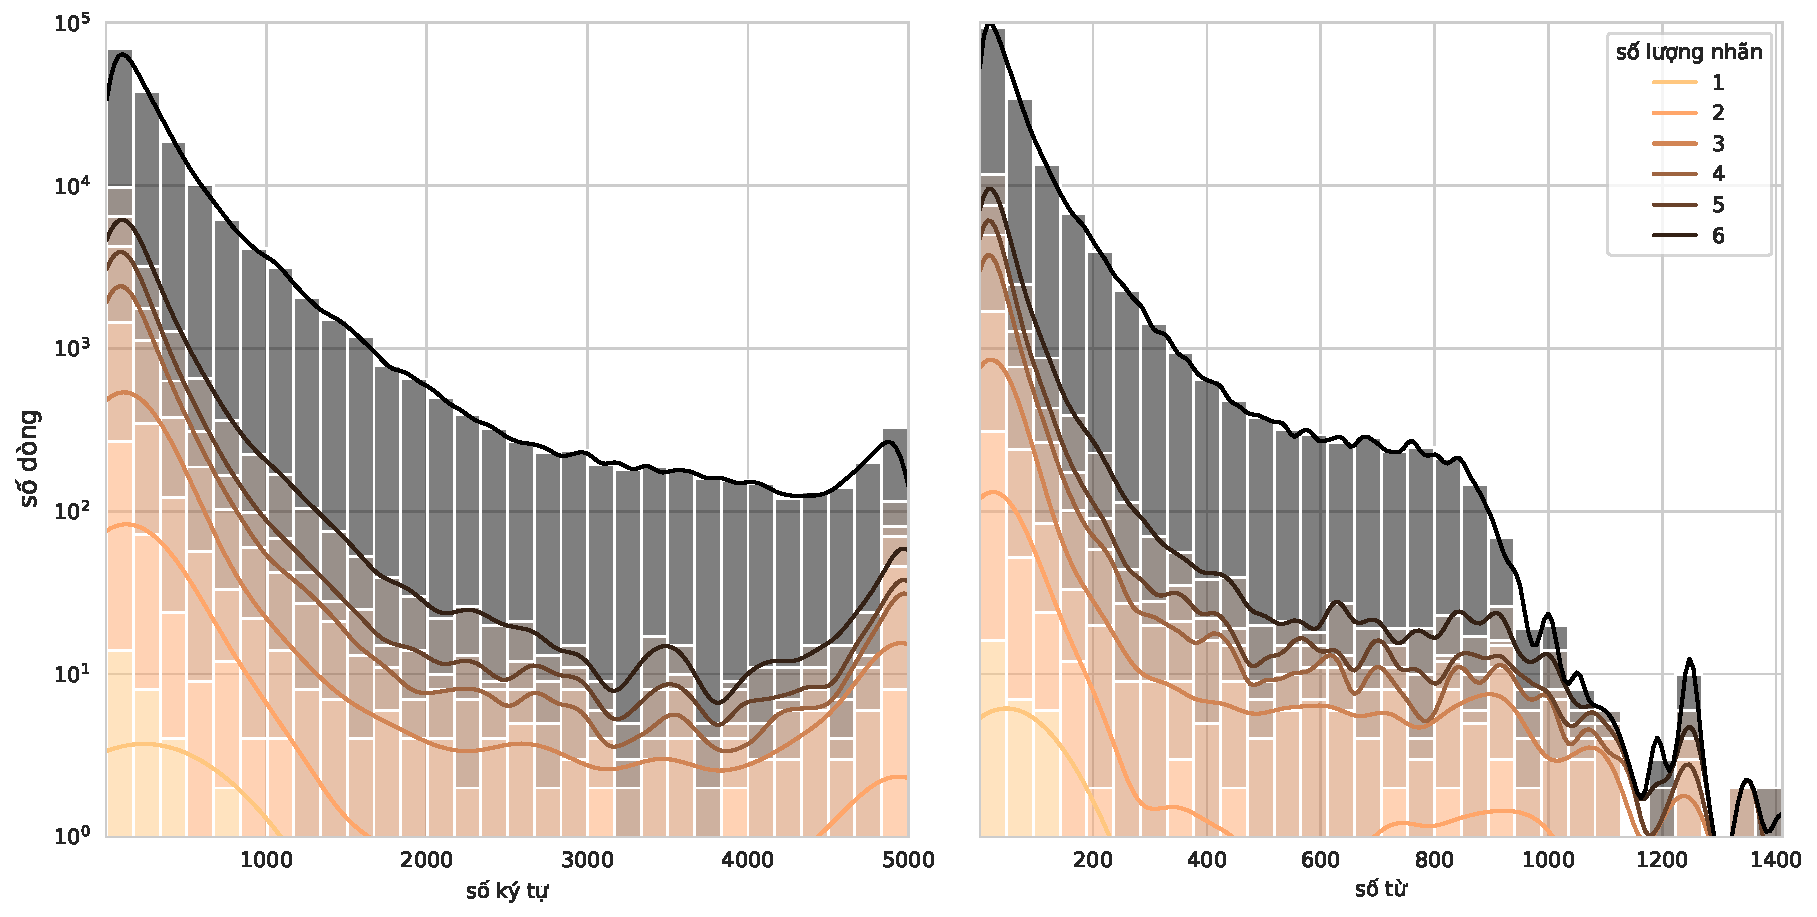
\includegraphics[width=\textwidth]{chapter_2/image/dist_num_chars_and_words_per_num_labels.pdf}
    \caption{Phân bố dữ liệu theo số nhãn, số ký tự và số từ}
\end{figure}

Có thể thấy phân bố dữ liệu theo thuộc tính ``có nhãn?'', hoặc theo ``số lượng nhãn'', theo một cách nào đó là khá tương đồng với nhau. Chỉ có một ngoại lệ, là phân bố theo số từ đối với dữ liệu không có nhãn, là rất thấp khi số lượng từ vượt qua $1000$.

Đối với phân bố dữ liệu theo từng loại nhãn đối với số ký tự, hay số từ là khá giống nhau.
\begin{figure}[htb]
    \centering
    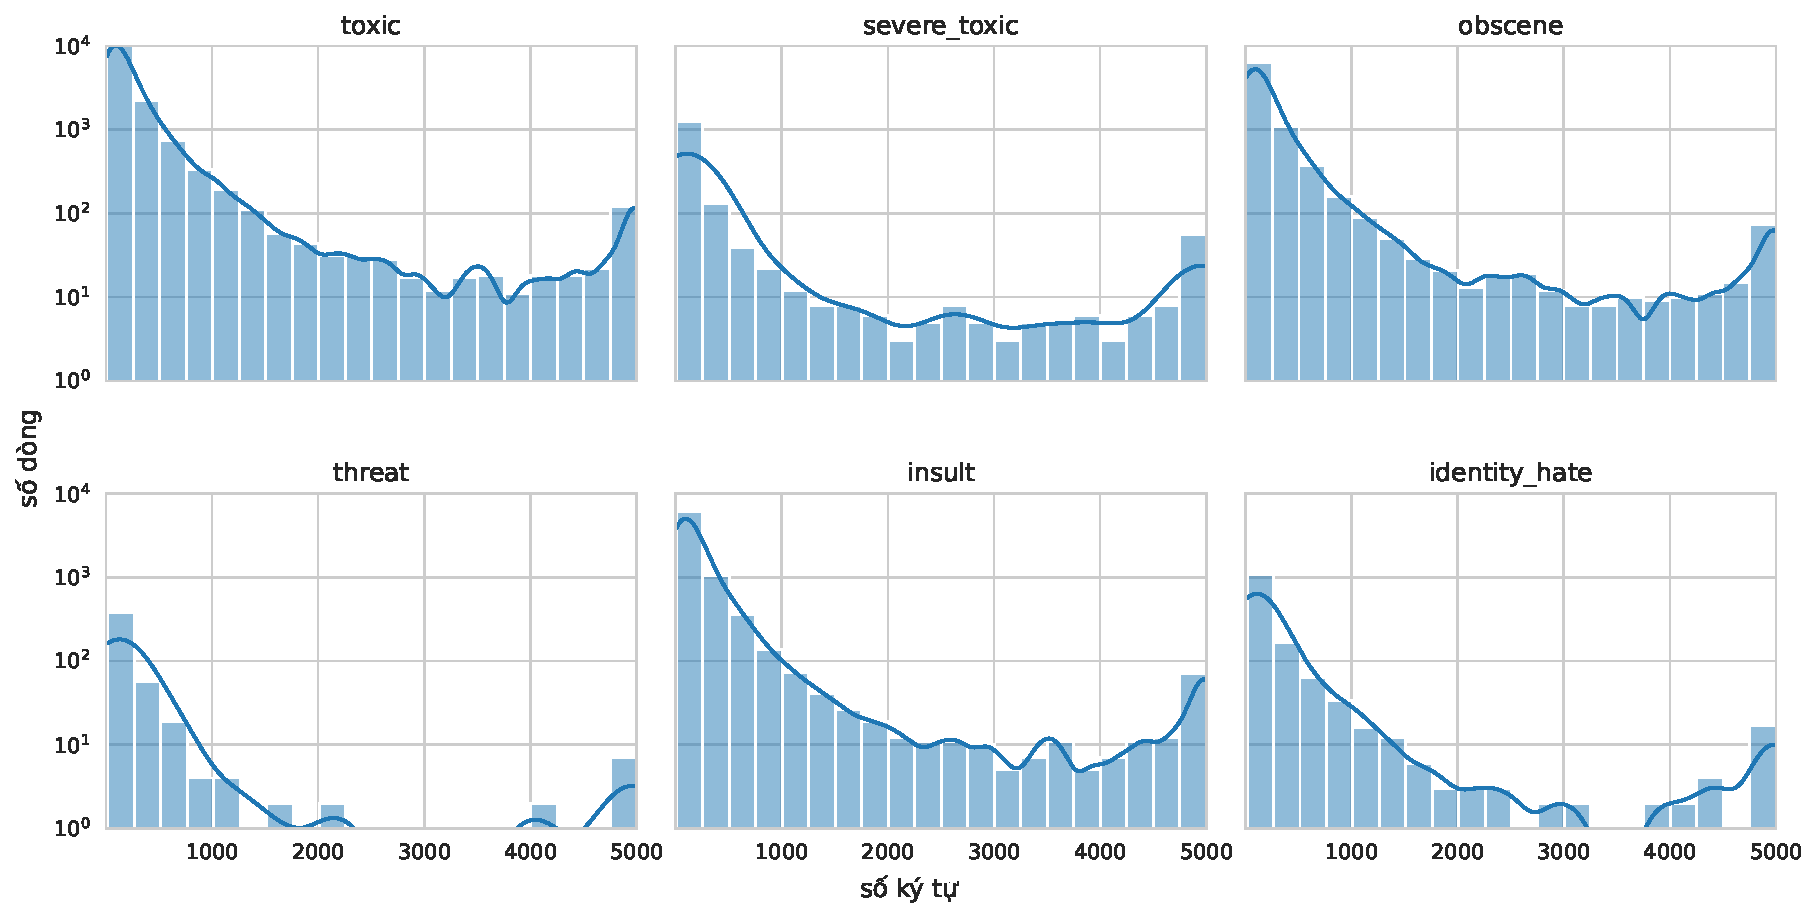
\includegraphics[width=\textwidth]{chapter_2/image/dist_num_chars_per_label.pdf}
    \caption{Phân bố dữ liệu đối với từng nhãn theo số ký tự}
\end{figure}
\begin{figure}[htb]
    \centering
    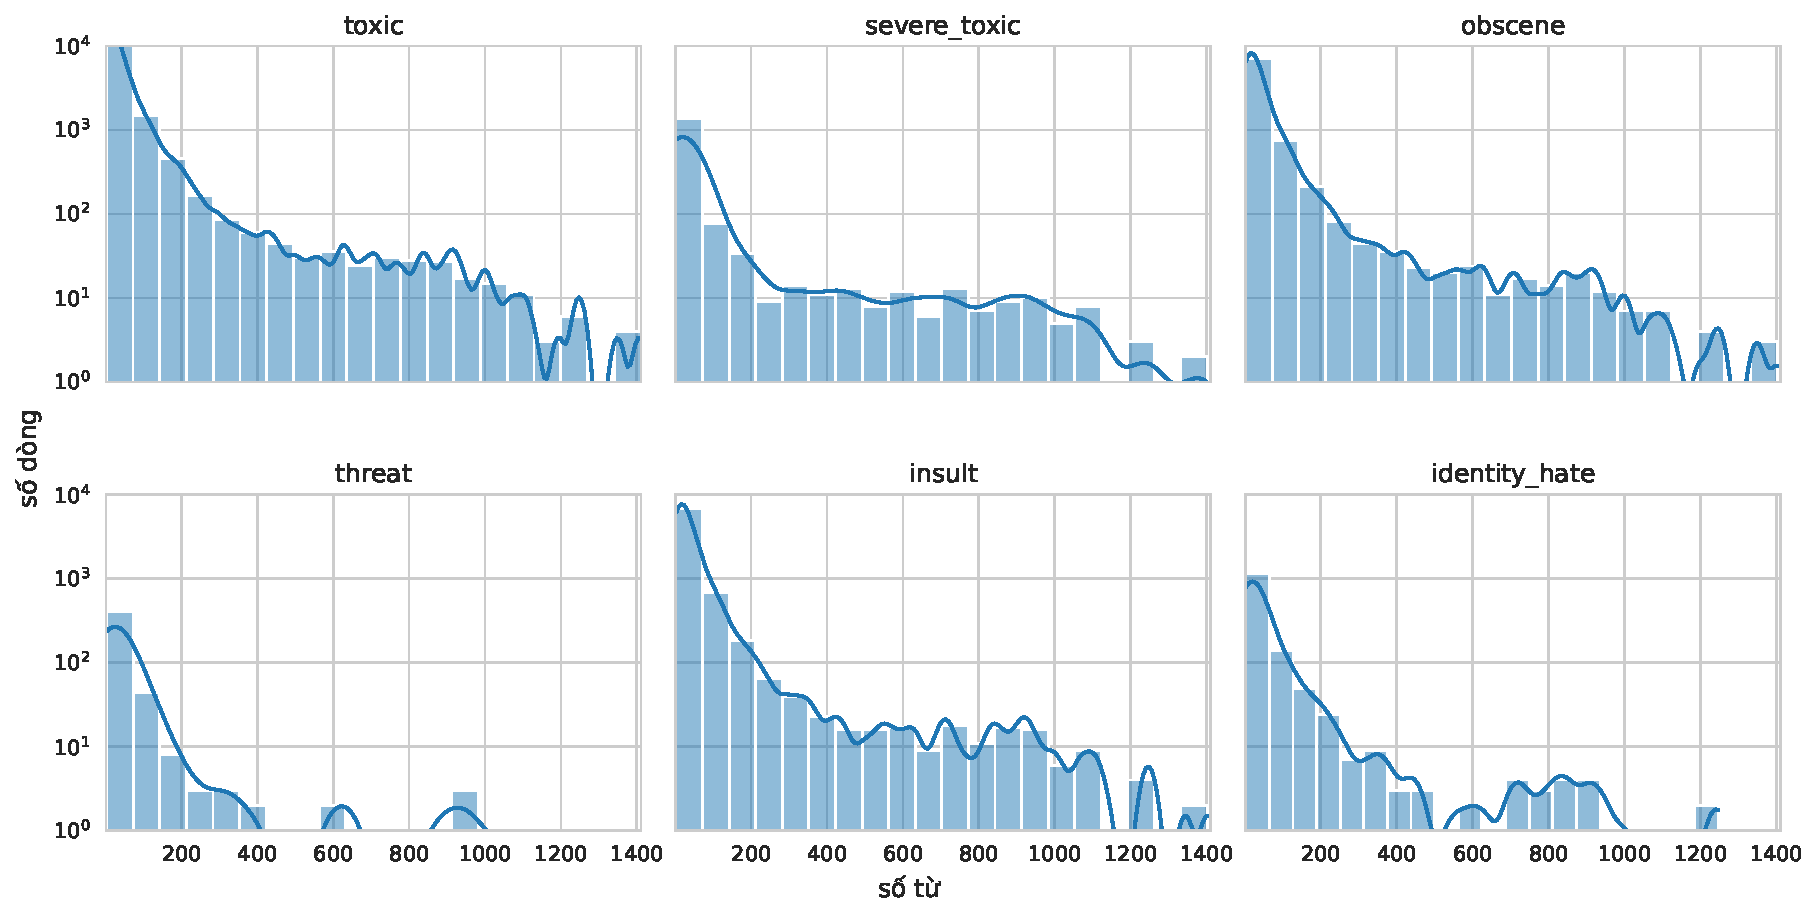
\includegraphics[width=\textwidth]{chapter_2/image/dist_num_words_per_label.pdf}
    \caption{Phân bố dữ liệu đối với từng nhãn theo số từ}
\end{figure}

Khi nhãn toxic là $0$, có rất ít dữ liệu thuộc các nhãn còn lại; khi các nhãn khác là $0$, nhãn toxic vẫn chiếm tỷ lệ rất lớn. Điều đó cho thấy nhãn toxic có thể được xem là nhãn tổng quát cho các nhãn còn lại. Nhãn severe\_toxic và nhãn threat chiếm tỉ trong rất nhỏ khi các nhãn còn lại bằng $0$, điều này một phần là do tỷ lệ hai loại nhãn này trong tập dữ liệu là rất thấp, nhưng cũng có khả năng những câu mang tính đe dọa nghiêm trọng thường không xuất hiện nhiều trong môi trường như Wikipedia.
\begin{figure}[htb]
    \centering
    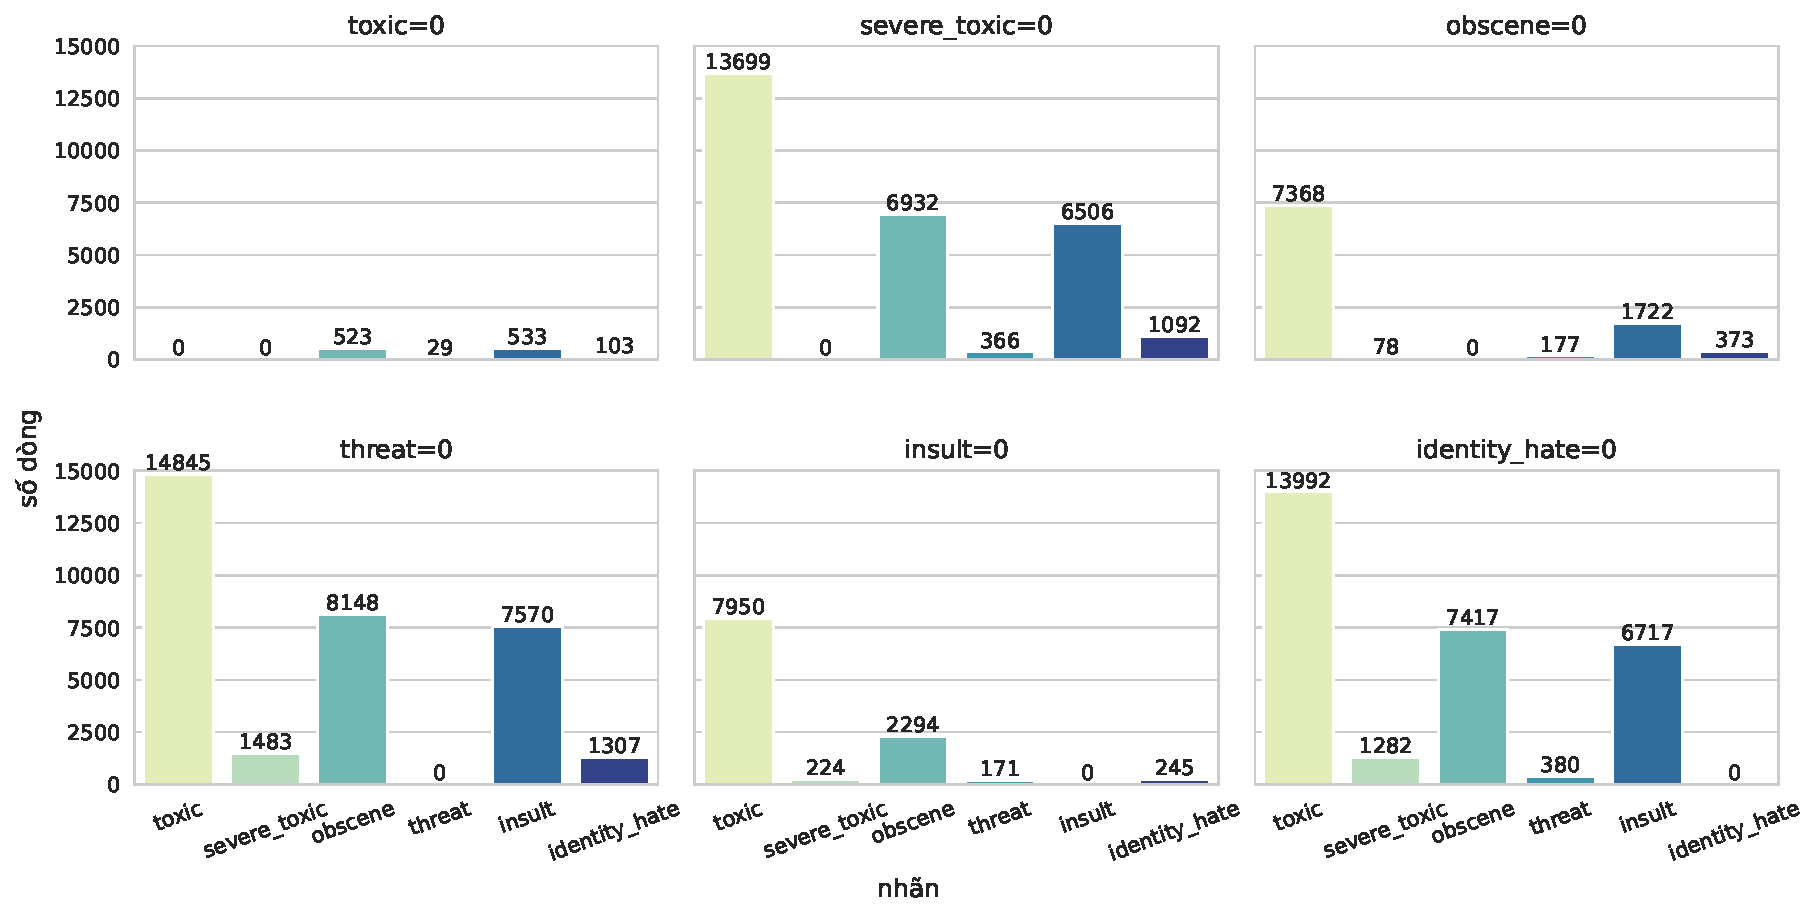
\includegraphics[width=\textwidth]{chapter_2/image/num_records_per_label_without_one_label.pdf}
    \caption{Phân bố dữ liệu đối với từng nhãn khi một nhãn bất kỳ là $0$}
\end{figure}
\clearpage

\section{Dữ liệu huấn luyện}
\begin{center}
    \textcolor{orange}{\faExclamationTriangle\. CẢNH BÁO: Bắt đầu từ đây sẽ có nhiều từ ngữ được xem là xúc phạm.}
\end{center}
\begin{table}[htb!]
    \rotatebox{90}{%
        \begin{minipage}{0.88\textheight}
            \centering
            \caption{Mẫu dữ liệu tiếng Anh (32 dòng)}
            \label{table:dataset-english}
            \RemoveFromHook{env/tabularx/before}[fontsize]
            \fontsize{8pt}{12pt}\selectfont
            \begin{threeparttable}
                \begin{tabularx}{\textwidth}{L{0.95} L{6.25} C{0.135} C{0.135} C{0.135} C{0.135} C{0.135} C{0.135}}
                    \toprule
                    \textbf{id}      & \textbf{comment\_text}                                                                                                           & \textbf{L1} & \textbf{L2} & \textbf{L3} & \textbf{L4} & \textbf{L5} & \textbf{L6} \\\midrule
                    0002bcb3da6cb337 & COCKSUCKER BEFORE YOU PISS AROUND ON MY WORK                                                                                     & \textit{1}  & \textit{1}  & \textit{1}  & 0           & \textit{1}  & 0           \\
                    00190820581d90ce & FUCK YOUR FILTHY MOTHER IN THE ASS, DRY!                                                                                         & \textit{1}  & 0           & \textit{1}  & 0           & \textit{1}  & 0           \\
                    0020e7119b96eeeb & Stupid peace of shit stop deleting my stuff asshole go die and fall in a hole go to hell!                                        & \textit{1}  & \textit{1}  & \textit{1}  & 0           & \textit{1}  & 0           \\
                    0020fd96ed3b8c8b & =Tony Sidaway is obviously a fistfuckee. He loves an arm up his ass.                                                             & \textit{1}  & 0           & \textit{1}  & 0           & \textit{1}  & 0           \\
                    003217c3eb469ba9 & Hi! I am back again!\textbackslash nLast warning!\textbackslash nStop undoing my edits or die!                                   & \textit{1}  & 0           & 0           & \textit{1}  & 0           & 0           \\
                    0036621e4c7e10b5 & Would you both shut up, you don't run wikipedia, especially a stupid kid.                                                        & \textit{1}  & 0           & 0           & 0           & \textit{1}  & 0           \\
                    00472b8e2d38d1ea & A pair of jew-hating weiner nazi schmucks.                                                                                       & \textit{1}  & 0           & \textit{1}  & 0           & \textit{1}  & \textit{1}  \\
                    006e87872c8b370c & you are a stupid fuck \textbackslash nand your mother's cunt stinks                                                              & \textit{1}  & \textit{1}  & \textit{1}  & 0           & \textit{1}  & 0           \\
                    0086998b34865f93 & Fuck you, block me, you faggot pussy!                                                                                            & \textit{1}  & 0           & \textit{1}  & 0           & \textit{1}  & 0           \\
                    0097dd5c29bf7a15 & u r a tw@ fuck off u gay boy.U r smelly.Fuck ur mum poopie                                                                       & \textit{1}  & 0           & \textit{1}  & 0           & \textit{1}  & \textit{1}  \\
                    00be7dcac98dc95d & this user is such a worthless goddamn faggot fuck you faggot                                                                     & \textit{1}  & 0           & \textit{1}  & 0           & \textit{1}  & 0           \\
                    00c0b8ed05ed7833 & Fuck off\textbackslash nYou are NOT an administrator. You DON'T have the authority to tell me what to do.                        & \textit{1}  & 0           & \textit{1}  & 0           & 0           & 0           \\
                    00c59720428c985a & ``\textbackslash n Fuck you \textbackslash n Fuck you award go fuck yourself ''                                                  & \textit{1}  & 0           & \textit{1}  & 0           & \textit{1}  & 0           \\
                    00d1d2f4f247d472 & MATT HARDY IS SO FUCKY!!!''Italic text[[Media:Example.ogg]]'''''MATT HARDY IS SO FUCKY!!!                                        & \textit{1}  & 0           & \textit{1}  & 0           & 0           & 0           \\
                    00dc0760994133ff & Fuck you \textbackslash n-User:The Bohemian Shinobis yeah, that's right, bitch! You are all pieces of shit!                      & \textit{1}  & 0           & \textit{1}  & 0           & \textit{1}  & 0           \\
                    01166f26ee280e56 & Gay \textbackslash nThe existence of CDVF is further proof that is a sad twat. He is also very ugly, and has a willy for a face. & \textit{1}  & 0           & \textit{1}  & 0           & \textit{1}  & \textit{1}  \\
                    011e2c96cfa8a055 & Fucked with the wrong muchacho. 21:19, July 23, 2005 (UTC)                                                                       & \textit{1}  & 0           & \textit{1}  & 0           & 0           & 0           \\
                    01208d2b76624130 & Hi \textbackslash nIm a fucking bitch.\textbackslash n50.180.208.181                                                             & \textit{1}  & \textit{1}  & \textit{1}  & 0           & \textit{1}  & 0           \\
                    014c96f873db11ff & ``````Nazi filth'''' is impolite 04:27, 20 Jan 2004 (UTC)\textbackslash n''                                                      & \textit{1}  & 0           & 0           & 0           & \textit{1}  & 0           \\
                    015c99386399aa14 & HELLO HOW DO I GET SOMEBODY TO FIX SHIT AROUND HERE?                                                                             & \textit{1}  & 0           & \textit{1}  & 0           & 0           & 0           \\
                    018663f910e0bfe6 & What a motherfucking piece of crap those fuckheads for blocking us!                                                              & \textit{1}  & \textit{1}  & \textit{1}  & 0           & \textit{1}  & 0           \\
                    018942e044417b74 & You sir are an imbecile, and a pervert.                                                                                          & \textit{1}  & 0           & 0           & 0           & \textit{1}  & 0           \\
                    019ab9a91e7fcdbe & Are you fucker mother fucker have nothing to do but block University computers. Go and suck cocks                                & \textit{1}  & 0           & \textit{1}  & 0           & \textit{1}  & 0           \\
                    01b1926bc5c1cc78 & IT WASNT VANDALISM, DICKHEAD                                                                                                     & \textit{1}  & 0           & \textit{1}  & 0           & \textit{1}  & 0           \\
                    01b9aa85cc61c03f & ``\textbackslash n You Suck \textbackslash nIf you don't undelete the page ````Barry Dejay'''' I will \%\$\#@ you!''             & \textit{1}  & 0           & \textit{1}  & 0           & \textit{1}  & 0           \\
                    01f467f73fb47c3e & You really are a rebel guy, rebelguys! \textbackslash nTime to get oral from a prostitute'''!                                    & \textit{1}  & 0           & 0           & 0           & \textit{1}  & 0           \\
                    0207005a6576eafc & Here's an idea \textbackslash nGo fuck yourself, cumshitter.                                                                     & \textit{1}  & \textit{1}  & \textit{1}  & 0           & \textit{1}  & 0           \\
                    02230885017a50c5 & Fuck you, Smith. Please have me notified when you die. I want to dance on your grave.                                            & \textit{1}  & 0           & \textit{1}  & \textit{1}  & \textit{1}  & 0           \\
                    022509df20736807 & I shit on your face \textbackslash nfuck you                                                                                     & \textit{1}  & 0           & \textit{1}  & 0           & \textit{1}  & 0           \\
                    02266b7fc5746618 & You are \textbackslash nso retarded.                                                                                             & \textit{1}  & 0           & 0           & 0           & \textit{1}  & 0           \\
                    023d01990e18a4da & HE LIKES ITIN THE ASS BY MUHAMAD ALI AND KELLY HAS A GIANT PENIS AND ALSO FUCKED COLUMBUS                                        & \textit{1}  & 0           & \textit{1}  & 0           & \textit{1}  & 0           \\
                    0265bcade39daa25 & Fuck off you murdering scum!!!                                                                                                   & \textit{1}  & 0           & \textit{1}  & 0           & \textit{1}  & 0           \\
                    \bottomrule
                \end{tabularx}
                \begin{tablenotes}
                    \fontsize{8pt}{12pt}\selectfont
                    \item \textbf{L1, L2, L3, L4, L5, L6} lần lượt là các nhãn \textbf{toxic, severe\_toxic, obscene, threat, insult, identity\_hate}
                \end{tablenotes}
            \end{threeparttable}
        \end{minipage}%
    }
\end{table}

Tập dữ liệu tiếng Anh sau khi được xử lý sẽ được dịch thành tập dữ liệu tiếng Việt, có mẫu như sau:
\begin{table}[htb!]
    \rotatebox{90}{%
        \begin{minipage}{0.88\textheight}
            \centering
            \caption{Mẫu dữ liệu tiếng Việt (32 dòng)}
            \label{table:dataset-vietnamese}
            \RemoveFromHook{env/tabularx/before}[fontsize]
            \fontsize{8pt}{12pt}\selectfont
            \begin{threeparttable}
                \begin{tabularx}{\textwidth}{L{0.95} L{6.25} C{0.135} C{0.135} C{0.135} C{0.135} C{0.135} C{0.135}}
                    \toprule
                    \textbf{id}      & \textbf{comment\_text}                                                                                                            & \textbf{L1} & \textbf{L2} & \textbf{L3} & \textbf{L4} & \textbf{L5} & \textbf{L6} \\\midrule
                    0002bcb3da6cb337 & đồ khốn nạn trước khi đi tiểu vào công việc của tôi                                                                               & \textit{1}  & \textit{1}  & \textit{1}  & 0           & \textit{1}  & 0           \\
                    00190820581d90ce & Đụ mẹ bẩn thỉu của ngươi vào mông đi , khô khan !                                                                                 & \textit{1}  & 0           & \textit{1}  & 0           & \textit{1}  & 0           \\
                    0020e7119b96eeeb & ngu ngốc yên bình chết tiệt đừng xóa đồ của tôi nữa đồ khốn kiếp đi chết và rơi xuống hố đi xuống địa ngục đi !                   & \textit{1}  & \textit{1}  & \textit{1}  & 0           & \textit{1}  & 0           \\
                    0020fd96ed3b8c8b & = tony sid a way rõ ràng là một tay đấm ee . Anh ấy thích một tay ôm mông mình .                                                  & \textit{1}  & 0           & \textit{1}  & 0           & \textit{1}  & 0           \\
                    003217c3eb469ba9 & xin chào ! tôi đã quay lại lần cuối . Cảnh báo lần cuối là đừng hoàn tác các chỉnh sửa của tôi nếu không sẽ chết !                & \textit{1}  & 0           & 0           & \textit{1}  & 0           & 0           \\
                    0036621e4c7e10b5 & Cả hai có thể im đi không , đừng chạy wikipedia , đặc biệt là một đứa trẻ ngu ngốc                                                & \textit{1}  & 0           & 0           & 0           & \textit{1}  & 0           \\
                    00472b8e2d38d1ea & một cặp người Do Thái ghét Weiner nazi schmucks .                                                                                 & \textit{1}  & 0           & \textit{1}  & 0           & \textit{1}  & \textit{1}  \\
                    006e87872c8b370c & Mày là một tên ngu ngốc và mẹ mày là cái lồn hôi hám                                                                              & \textit{1}  & \textit{1}  & \textit{1}  & 0           & \textit{1}  & 0           \\
                    0086998b34865f93 & Mẹ kiếp , chặn tao lại , đồ khốn nạn !                                                                                            & \textit{1}  & 0           & \textit{1}  & 0           & \textit{1}  & 0           \\
                    0097dd5c29bf7a15 & ura tw @ chết tiệt đi cậu bé đồng tính của cậu ( url ) mẹ cậu là poo pie                                                          & \textit{1}  & 0           & \textit{1}  & 0           & \textit{1}  & \textit{1}  \\
                    00be7dcac98dc95d & người dùng này đúng là một tên khốn vô dụng , đồ khốn kiếp                                                                        & \textit{1}  & 0           & \textit{1}  & 0           & \textit{1}  & 0           \\
                    00c0b8ed05ed7833 & chết tiệt , bạn không phải là quản trị viên . Bạn không có quyền bảo tôi phải làm gì .                                            & \textit{1}  & 0           & \textit{1}  & 0           & 0           & 0           \\
                    00c59720428c985a & chết tiệt , đồ khốn , giải thưởng hãy đi chết tiệt đi                                                                             & \textit{1}  & 0           & \textit{1}  & 0           & \textit{1}  & 0           \\
                    00d1d2f4f247d472 & Matt Hardy thật là một phương tiện truyền thông văn bản in nghiêng : ( url ) ] ] ' ' ' ' một Matt Hardy thật là chết tiệt y ! ! ! & \textit{1}  & 0           & \textit{1}  & 0           & 0           & 0           \\
                    00dc0760994133ff & fuck you - người dùng shin shin bohemian vâng , đúng vậy , con khốn ! tất cả các bạn đều là đồ khốn nạn !                         & \textit{1}  & 0           & \textit{1}  & 0           & \textit{1}  & 0           \\
                    01166f26ee280e56 & gay sự tồn tại của cd vf là một bằng chứng nữa cho thấy đó là một gã khốn nạn . Anh ta cũng rất xấu xí và có khuôn mặt u ám .     & \textit{1}  & 0           & \textit{1}  & 0           & \textit{1}  & \textit{1}  \\
                    011e2c96cfa8a055 & thật sai lầm . ( thời gian ) , ngày 23 tháng 7 năm 2005 ( utc )                                                                   & \textit{1}  & 0           & \textit{1}  & 0           & 0           & 0           \\
                    01208d2b76624130 & xin chào tôi là con khốn nạn . ( địa chỉ IP )                                                                                     & \textit{1}  & \textit{1}  & \textit{1}  & 0           & \textit{1}  & 0           \\
                    014c96f873db11ff & `` `` `` sự bẩn thỉu của Đức Quốc xã '' '' là bất lịch sự ( thời gian ) , ngày 20 tháng 1 năm 2004 ( utc ) ''                     & \textit{1}  & 0           & 0           & 0           & \textit{1}  & 0           \\
                    015c99386399aa14 & Xin chào , làm cách nào để tôi nhờ ai đó sửa chữa thứ rác rưởi quanh đây ?                                                        & \textit{1}  & 0           & \textit{1}  & 0           & 0           & 0           \\
                    018663f910e0bfe6 & thật là một thứ khốn kiếp , những cái đầu chết tiệt đó đã chặn chúng ta !                                                         & \textit{1}  & \textit{1}  & \textit{1}  & 0           & \textit{1}  & 0           \\
                    018942e044417b74 & Thưa ngài , ngài là một kẻ ngu ngốc và hư hỏng .                                                                                  & \textit{1}  & 0           & 0           & 0           & \textit{1}  & 0           \\
                    019ab9a91e7fcdbe & mày có phải đồ khốn không , đồ khốn , không có việc gì làm ngoài chặn máy tính của trường đại học . Đi mà bú cặc đi               & \textit{1}  & 0           & \textit{1}  & 0           & \textit{1}  & 0           \\
                    01b1926bc5c1cc78 & Đó không phải là phá hoại đâu , đồ khốn                                                                                           & \textit{1}  & 0           & \textit{1}  & 0           & \textit{1}  & 0           \\
                    01b9aa85cc61c03f & `` thật tệ nếu bạn không xóa trang `` `` barry de jay '' '' tôi sẽ \% ( đô la ) \# @ bạn ! ''                                     & \textit{1}  & 0           & \textit{1}  & 0           & \textit{1}  & 0           \\
                    01f467f73fb47c3e & Mày đúng là một kẻ nổi loạn , những kẻ nổi loạn ! đã đến lúc nhận lời của một gái điếm ' ' ' !                                    & \textit{1}  & 0           & 0           & 0           & \textit{1}  & 0           \\
                    0207005a6576eafc & Đây là một ý kiến hay , đi chết tiệt đi , kẻ đánh người .                                                                         & \textit{1}  & \textit{1}  & \textit{1}  & 0           & \textit{1}  & 0           \\
                    02230885017a50c5 & Mẹ kiếp , Smith . Làm ơn cho tôi biết khi nào bạn chết . Tôi muốn nhảy múa trên mộ bạn .                                          & \textit{1}  & 0           & \textit{1}  & \textit{1}  & \textit{1}  & 0           \\
                    022509df20736807 & tôi ị vào mặt cậu chết tiệt                                                                                                       & \textit{1}  & 0           & \textit{1}  & 0           & \textit{1}  & 0           \\
                    02266b7fc5746618 & bạn thật chậm chạp .                                                                                                              & \textit{1}  & 0           & 0           & 0           & \textit{1}  & 0           \\
                    023d01990e18a4da & anh ấy thích nó vào mông bởi muha mad ali và kelly có một dương vật khổng lồ và cũng đụ columbus                                  & \textit{1}  & 0           & \textit{1}  & 0           & \textit{1}  & 0           \\
                    0265bcade39daa25 & Cút đi tên sát nhân cặn bã ! ! !                                                                                                  & \textit{1}  & 0           & \textit{1}  & 0           & \textit{1}  & 0           \\
                    \bottomrule
                \end{tabularx}
                \begin{tablenotes}
                    \fontsize{8pt}{12pt}\selectfont
                    \item \textbf{L1, L2, L3, L4, L5, L6} lần lượt là các nhãn \textbf{toxic, severe\_toxic, obscene, threat, insult, identity\_hate}
                \end{tablenotes}
            \end{threeparttable}
        \end{minipage}%
    }
\end{table}
\clearpage

\section{Dữ liệu bên lề}
\subsection*{Từ viết tắt trong tiếng Anh (\textit{abbreviation})\footnote{\url{https://www.grammarly.com/blog/types-abbreviations/}}}
\begin{table}[htb]
    \centering
    \caption{Một vài từ viết tắt dạng \textit{contraction}}
    \label{table:english-contractions}
    \begin{tabular}{ll}
        \toprule
        \textbf{Từ viết tắt} & \textbf{Từ hoàn chỉnh} \\\midrule
        won't                & will not               \\
        can't                & can not                \\
        n't                  & not                    \\
        're                  & are                    \\
        's                   & is                     \\
        'd                   & would                  \\
        'll                  & will                   \\
        't                   & not                    \\
        've                  & have                   \\
        'm                   & am                     \\
        \bottomrule
    \end{tabular}
\end{table}
Đối với các từ viết tắt dạng \textit{clipping}, \textit{initialism}, \textit{acronym} và \textit{textese}, nhóm quyết định không thay thế chúng mà để cho mô hình nhúng từ xử lý chúng.
\begin{table}[htb]
    \centering
    \caption{Các cụm từ viết tắt khác}
    \begin{tabular}{lll}
        \toprule
        \textbf{Dạng}               & \textbf{Từ viết tắt} & \textbf{Từ hoàn chỉnh}                        \\\midrule
        \multirow{2}{*}{clipping}   & ad                   & advertisement                                 \\
                                    & app                  & application                                   \\\midrule
        \multirow{2}{*}{initialism} & FBI                  & Federal Bureau of Investigation               \\
                                    & UFO                  & Unidentified Flying Object                    \\\midrule
        \multirow{2}{*}{acronym}    & PIN                  & Personal Identification Number                \\
                                    & NASA                 & National Aeronautics and Space Administration \\\midrule
        \multirow{2}{*}{textese}    & lol                  & laugh out loud                                \\
                                    & btw                  & by the way                                    \\
        \bottomrule
    \end{tabular}
\end{table}
\clearpage

\subsection*{English Letter Frequency Counts\footnote{\url{https://norvig.com/mayzner.html}}}
Biểu đồ tần suất của 2 từ liền kề (\textit{bigram}) trong tiếng Anh.
\begin{figure}[htb]
    \centering
    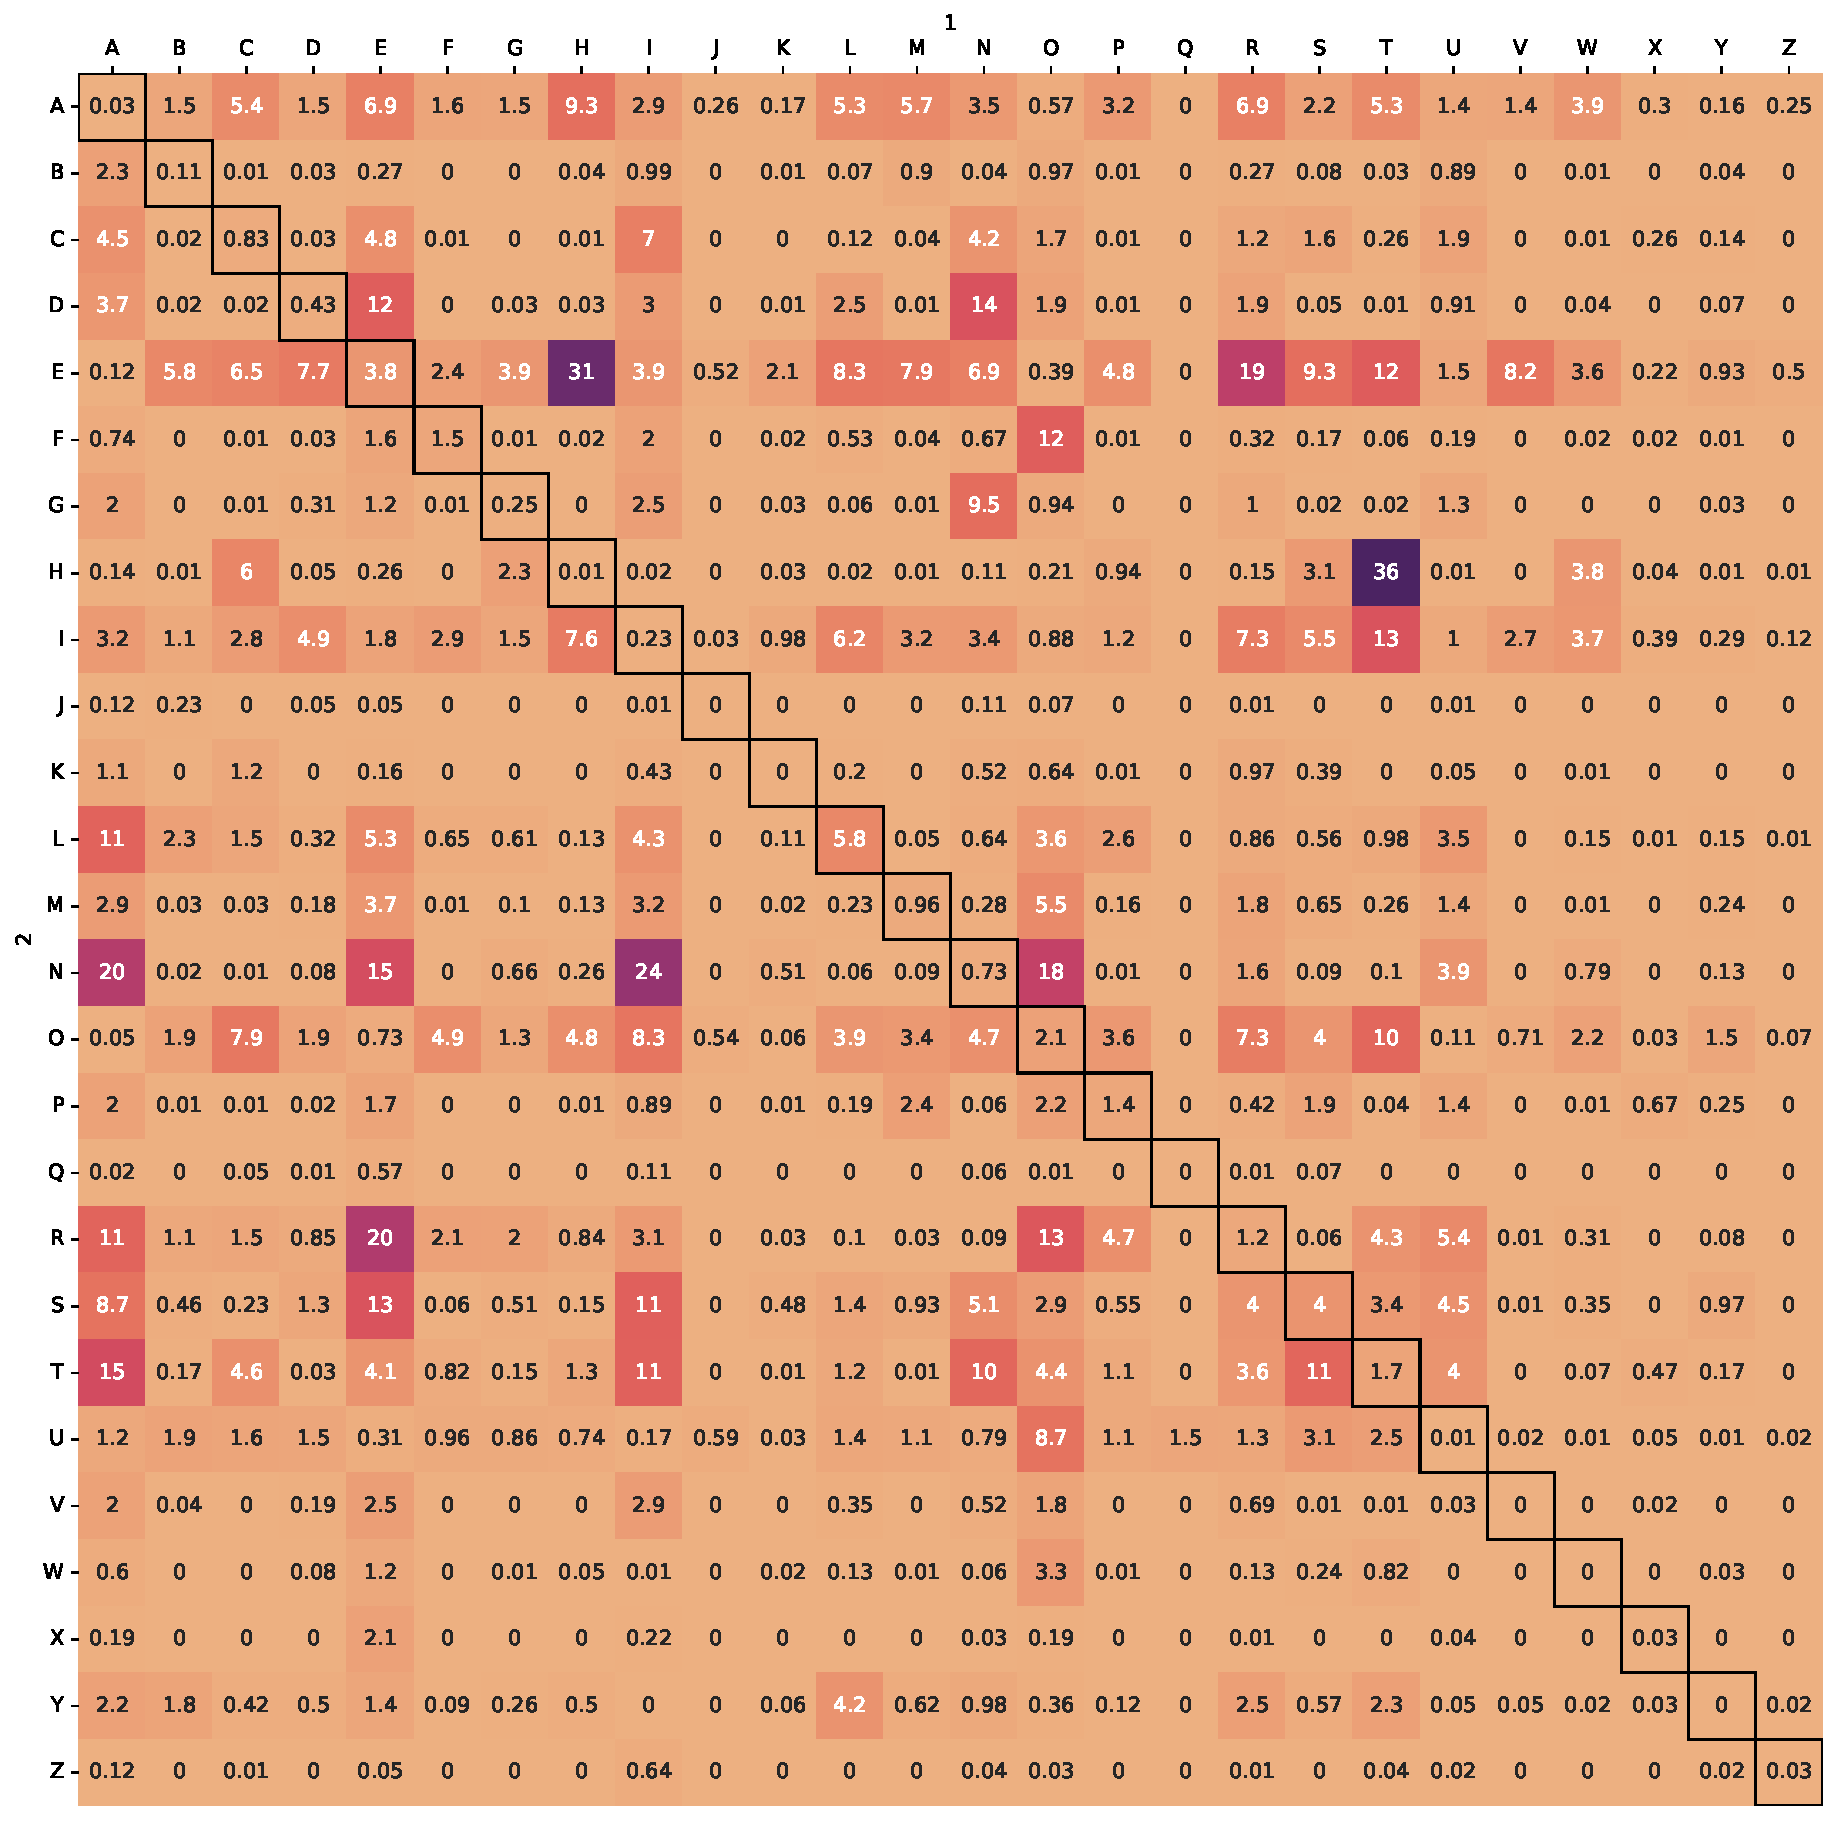
\includegraphics[width=\textwidth]{chapter_2/image/norvig_bigram_frequency.pdf}
    \caption{Biểu đồ tần suất 2 từ liền kề trong tiếng Anh (đơn vị phần nghìn \textperthousand)}
    \label{figure:english_bigram_frequency}
\end{figure}

\newpage
\subsection*{Dữ liệu liên quan đến Wikipedia}
\begin{table}[htb]
    \centering
    \caption{Một vài phím tắt đặc biệt của Wikipedia}
    \label{table:wikipedia-shortcuts}
    \begin{tabular}{l l}
        \toprule
        \textbf{Tên}                                                    & \textbf{shortcut} \\\midrule
        \multirow{6}{*}{\texttt{wikipedia shortcut\footnotemark}}       & Portal:Contents   \\
                                                                        & WP:QI             \\
                                                                        & WP:TI             \\
                                                                        & P:LIT             \\
                                                                        & WP:MOS-ZH         \\
                                                                        & \dots             \\\midrule
        \multirow{4}{*}{\texttt{wikipedia namespace\footnotemark}}      & WP:\              \\
                                                                        & Project:\_        \\
                                                                        & Project talk:\_   \\
                                                                        & \dots             \\\midrule
        \multirow{3}{*}{\texttt{wikipedia file namespace\footnotemark}} & Image:\_          \\
                                                                        & Image talk:\_     \\
                                                                        & \dots             \\
        \bottomrule
    \end{tabular}
\end{table}
\footnotetext[2]{\url{https://en.wikipedia.org/wiki/Wikipedia:Shortcut\_index}}
\footnotetext[3]{\url{https://en.wikipedia.org/wiki/Wikipedia:Namespace}}
\footnotetext[4]{\url{https://en.wikipedia.org/wiki/Wikipedia:Namespace}}

\newpage
\subsection*{Dữ liệu liên quan đến Unicode}
Bảng mã Unicode có rất nhiều khối\footnote{\url{https://www.compart.com/en/unicode/block}} khác nhau, nhưng phần lớn trong đó là các ký tự của các ngôn ngữ trên thế giới.
\begin{table}[htb]
    \centering
    \caption{Các khối Unicode được sử dụng}
    \label{table:unicode-blocks}
    \begin{threeparttable}
        \begin{tabular}{llccc}
            \toprule
            \multirow{2}{*}{\textbf{Loại}} & \multirow{2}{*}{\textbf{Tên khối}}      & \multicolumn{2}{c}{\textbf{Khoảng Unicode}} & \multirow{2}{*}{ \textbf{Ví dụ}}     \\\cmidrule(lr){3-4}
                                           &                                         & Bắt đầu                                     & Kết thúc                         &   \\\midrule
            \multirow{8}{*}{Latin}         & Basic Latin                             & U+0000                                      & U+007F                           & a \\
                                           & Latin-1 Supplement                      & U+0080                                      & U+00FF                           & á \\
                                           & Latin Extended-A                        & U+0100                                      & U+017F                           & ă \\
                                           & Latin Extended-B                        & U+0180                                      & U+024F                           & ơ \\
                                           & Latin Extended Additional               & U+1E00                                      & U+1EFF                           & ả \\
                                           & Latin Extended-C                        & U+2C60                                      & U+2C7F                           & ⱽ \\
                                           & Latin Extended-D                        & U+A720                                      & U+A7FF                           & ꞷ \\
                                           & Latin Extended-E                        & U+AB30                                      & U+AB6F                           & ꬶ \\\midrule
            \multirow{4}{*}{Greek}         & Greek and Coptic                        & U+0370                                      & U+03FF                           & β \\
                                           & Greek Extend                            & U+1F00                                      & U+1FFF                           & ἀ \\
                                           & Ancient Greek Numbers\tnote{1}          & U+10140                                     & U+1018F                          &   \\
                                           & Ancient Greek Musical Notation\tnote{2} & U+1D200                                     & U+1D24F                          &   \\\midrule
            \multirow{3}{*}{Phonetic}      & Phonetic Extensions                     & U+1D00                                      & U+1D7F                           & ᴀ \\
                                           & Phonetic Extensions Supplement          & U+1D80                                      & U+1DBF                           & ᶆ \\
                                           & Katakana Phonetic Extensions\tnote{3}   & U+31F0                                      & U+31FF                           &   \\\midrule
            \multirow{3}{*}{Others}        & Spacing Modifier Letters                & U+02B0                                      & U+02FF                           & ʰ \\
                                           & General Punctuation                     & U+2000                                      & U+206F                           & ‚ \\
                                           & Currency Symbols                        & U+20A0                                      & U+20CF                           & € \\
            \bottomrule
        \end{tabular}
        \begin{tablenotes}
            \item [1] Chữ số của người Hy Lạp cổ.
            \item [2] Ký hiệu âm nhạc của người Hy Lạp cổ.
            \item [3] Chữ cái tiếng Nhật.
        \end{tablenotes}
    \end{threeparttable}
\end{table}

Nhóm nhận thấy, trong tập dữ liệu, các ký tự thuộc các ngôn ngữ như Trung, Hindi, Thái, Hàn, v.v. thường là các từ thuộc dạng spam và không mang nhiều ý nghĩa. Vì vậy nhóm đã quyết định loại bỏ hoàn toàn các ký tự như vậy, và tập trung vào xử lý các ký tự latin và một vài ký tự khác gần giống với ký tự latin.

\clearpage
Bảng mã Unicode có nhiều nhóm\footnote{\url{https://www.compart.com/en/unicode/category}} khác nhau, nhưng trong đề tài này chỉ tập trung vào xử lý các nhóm chính.
\begin{table}[htb]
    \centering
    \caption{Các nhóm Unicode}
    \label{table:unicode-categories}
    \begin{tabular}{llr}
        \toprule
        \textbf{Tên viết tắt} & \textbf{Mô tả}                   & \textbf{Ví dụ} \\\midrule
        L                     & Chữ cái                          & a              \\
        M                     & Các loại dấu thanh               & ◌́              \\
        N                     & Chữ số                           & 2              \\
        P                     & Dấu câu                          & ,              \\
        S                     & Ký hiệu, ký tự đặc biệt          & +              \\
        Z                     & Các loại khoảng trắng, ngắt dòng &                \\
        C                     & Các ký hiệu còn lại              &                \\
        \bottomrule
    \end{tabular}
\end{table}

Biến đổi các ký tự đặc biệt còn lại về bảng mã ASCII\footnote{\url{https://interglacial.com/tpj/22/}}.
\begin{table}[htb]
    \centering
    \caption{Một vài biến đổi giữa ký tự đặc biệt và ký tự ASCII}
    \label{table:deunicode}
    \begin{tabular}{ll}
        \toprule
        \textbf{Ký tự đặc biệt}     & \textbf{Ký tự ASCII} \\\midrule
        Æ                           & AE                   \\
        é                           & e                    \\
        {\fontspec{MS Gothic}北亰}    & Bei Jing             \\
        {\fontspec{MS Gothic}げんまい茶} & genmaiCha            \\
        {\fontspec{MS Gothic}δ}     & d                    \\
        \dots                       & \dots                \\
        \bottomrule
    \end{tabular}
\end{table}

Một vài ký tự đặc biệt khi biến đổi về dạng ASCII sẽ không giống hoặc không hoàn toàn giống với hình dạng của ký tự đó, ví dụ như:
\begin{itemize}
    \item Æ\textrightarrow AE, nhưng có thể là A hoặc E hoặc AE.
    \item Ἠ\textrightarrow E, nhưng có thể là H.
    \item v.v..
\end{itemize}

\newpage
\subsection*{Dữ liệu liên quan đến các loại emoticons/emojis}
Các emoticons được thu thập từ nhiều nguồn\footnote{\url{https://en.wikipedia.org/wiki/List\_of\_emoticons}, \url{https://github.com/jigglycrumb/ASCIImoji}, \url{https://github.com/dysfunc/ascii-emoji}, \url{https://emojidb.org/}} khác nhau.
\begin{table}[htb]
    \centering
    \caption{Một vài emoticons}
    \label{table:emoticons}
    \begin{tabular}{lll}
        \toprule
        \textbf{Emoticons}                & \textbf{Tên tiếng Anh}    & \textbf{Tên tiếng Việt}        \\\midrule
        {\fontspec{Consolas}:)}           & smiley, happy face        & khuôn mặt tươi cười, hạnh phúc \\
        {\fontspec{Consolas}xD}           & laughing                  & cười                           \\
        {\fontspec{Consolas}:-))}         & very happy or double chin & rất vui vẻ hoặc cằm đôi        \\
        {\fontspec{Consolas}8-X}          & skull and crossbones      & đầu lâu xương chéo             \\
        {\fontspec{Consolas}~:>}          & chicken                   & thịt gà                        \\
        {\fontspec{Consolas}@\};-}        & rose                      & hoa hồng                       \\
        {\fontspec{Consolas}8====D}       & penis, ejaculation        & dương vật, xuất tinh           \\
        {\fontspec{Consolas}( . Y . )}    & boobs                     & ngực                           \\
        {\fontspec{Consolas}( ° ͜ʖ͡°)╭∩╮}   & fuck                      & chết tiệt                      \\
        {\fontspec{Consolas}╭∩╮(-\_-)╭∩╮} & fuck                      & chết tiệt                      \\
        \dots                             & \dots                     & \dots                          \\
        \bottomrule
    \end{tabular}
\end{table}

\begin{table}[htb]
    \centering
    \caption[Một vài emojis]{Một vài emojis\footnotemark}
    \label{table:emojis}
    \begin{tabular}{lll}
        \toprule
        \textbf{emojis}                        & \textbf{Tên tiếng Anh}          & \textbf{Tên tiếng Việt}                       \\\midrule
        {\fontspec{Segoe UI Emoji}\char"1F600} & grinning face                   & khuôn mặt cười toe toét                       \\
        {\fontspec{Segoe UI Emoji}\char"1F603} & grinning face with big eyes     & khuôn mặt cười toe toét với đôi mắt to        \\
        {\fontspec{Segoe UI Emoji}\char"1F604} & grinning face with smiling eyes & khuôn mặt cười toe toét với đôi mắt biết cười \\
        {\fontspec{Segoe UI Emoji}\char"1F601} & beaming face with smiling eyes  & khuôn mặt rạng rỡ với đôi mắt biết cười       \\
        {\fontspec{Segoe UI Emoji}\char"1F606} & grinning squinting face         & mặt nhăn nhó cười toe toét                    \\
        {\fontspec{Segoe UI Emoji}\char"1F605} & grinning face with sweat        & mặt cười toe toét mồ hôi                      \\
        {\fontspec{Segoe UI Emoji}\char"1F923} & rolling on the floor laughing   & Cười lăn lộn                                  \\
        {\fontspec{Segoe UI Emoji}\char"1F602} & face with tears of joy          & khuôn mặt với giọt nước mắt của niềm vui      \\
        {\fontspec{Segoe UI Emoji}\char"1F642} & slightly smiling face           & khuôn mặt hơi mỉm cười                        \\
        {\fontspec{Segoe UI Emoji}\char"1F643} & upside-down face                & mặt lộn ngược                                 \\
        \dots                                  & \dots                           & \dots                                         \\
        \bottomrule
    \end{tabular}
\end{table}
\footnotetext{\url{https://unicode.org/Public/emoji/15.1/}}

\newpage
\subsection*{Dữ liệu về word embedding}
\begin{table}[htb]
    \centering
    \caption{Ví dụ về từ gần nhau khi dùng word embedding}
    \label{table:fasttext-mostsimilar}
    \begin{tabular}{l l c}
        \toprule
        \textbf{Đầu vào}        & \textbf{Đầu ra} & \textbf{Tần suất} \\\midrule
        \multirow{10}{*}{nhiều} & nhiềuu          & $0.9332$          \\
                                & nhiều-nhiều     & $0.9273$          \\
                                & nhiều-rất       & $0.8605$          \\
                                & một-nhiều       & $0.8106$          \\
                                & ta-nhiều        & $0.8099$          \\
                                & này-nhiều       & $0.8048$          \\
                                & nhiều-tính      & $0.7755$          \\
                                & nhiều-xin\_chào & $0.6692$          \\
                                & nhiều-người\_mỹ & $0.6597$          \\
                                & ít              & $0.6578$          \\\midrule
        \multirow{10}{*}{điên}  & điên\_điên      & $0.8487$          \\
                                & z\_điên         & $0.8201$          \\
                                & đá\_điên        & $0.7975$          \\
                                & mụ\_điên        & $0.7946$          \\
                                & phì\_điên       & $0.7862$          \\
                                & mũ\_điên        & $0.7792$          \\
                                & điên\_ocd       & $0.7778$          \\
                                & sủa\_điên       & $0.7620$          \\
                                & kẻ\_điên        & $0.7601$          \\
                                & lợn\_điên       & $0.7547$          \\
        \bottomrule
    \end{tabular}
\end{table}

\newpage
\subsection*{Các loại văn bản đặc biệt}\label{special-text}
Một ví dụ về văn bản chỉ có thể hiểu bằng cách nhìn

\begin{center}
    \begin{minipage}{0.4\textwidth}
        \fontspec{Segoe UI Symbol}
        \fontsize{6pt}{9pt}\selectfont
        ⠀⠀⠀⠀⠀⠀⠀⠀⠀⠀⠀⠀⠀⠀⣀⣀⣀⡀⠀⠀⠀⠀⠀⠀⠀⣀⣀⣀⣀⡀\\
        ⠀⠀⠀⠀⠀⠀⠀⠀⠀⠀⢀⡴⠞⠉⠉⠀⠀⠛⠉⢗⡦⣄⣴⠚⠉⠁⠀⠀⠀⠙⣷⣄\\
        ⠀⠀⠀⠀⠀⠀⠀⠀⢀⡴⠋⠀⠀⠀⢤⣀⡀⠀⣀⣰⣬⣿⣧⡠⠀⠀⠀⠀⠀⠀⡨⣿⣇\\
        ⠀⠀⠀⠀⠀⠀⠀⢠⡟⠁⠀⣠⣤⠾⠋⠀⠀⠀⠀⠀⠉⠙⠻⣞⣒⠒⠉⠉⠉⠉⠉⠉⠉⠛⠲⣦⡀\\
        ⠀⠀⠀⠀⠀⠀⢠⡟⠀⠀⠀⠉⠁⠀⠀⠀⣲⡭⣒⣒⠒⠦⢈⣉⣻⣿⣷⣿⣾⡢⠭⠭⠩⠭⠭⠽⢽⣶⡀\\
        ⠀⠀⠀⠀⣀⣤⣾⠁⠀⠀⠀⢀⣠⣤⢴⣻⡷⠛⢁⡀⠤⣀⡂⠤⠤⠼⢿⣯⣓⠤⠍⢒⡶⢶⣮⣍⠉⠘⠻⡀\\
        ⠀⠀⠀⡴⠛⣿⣿⠀⠀⠀⢰⣶⣛⣞⣛⡓⠶⠿⠒⣪⡛⣻⡿⢶⣄⠀⢸⠃⠀⠀⢀⣿⠶⣾⠉⣹⣧⣀⣴⠃\\
        ⠀⠀⣰⠅⠀⠙⠁⠀⠀⠀⠀⠁⠀⢠⣝⣷⣤⣄⣀⣿⣏⣹⣦⡾⠿⣾⣿⠒⠒⠒⠲⠛⠛⠉⠋⡁⣩⠟⠁\\
        ⠀⣰⠇⠀⠀⠀⠀⠀⠀⠀⠀⠀⠀⠈⠁⠈⠉⠓⠚⠒⠒⠚⢊⣱⠏⠉⠁⡤⣴⣄⣀⣀⣀⣰⣿⡟⠁\\
        ⠀⣿⠀⠀⠀⠀⠀⠀⠀⠀⠀⠀⠀⠀⠀⠀⠀⠀⢠⣠⠵⠚⠉⠁⠀⠀⠀⠀⠀⠉⠛⠉⠀⠀⠀⠙⢦\\
        ⢀⡇⠀⠀⠀⠀⠀⠀⠀⠀⠀⠀⠀⠀⠀⠀⠀⠀⠀⠀⠀⠀⠀⠀⠀⠀⠀⠀⠀⠀⠀⠀⠀⠀⠀⠀⢮⣧\\
        ⢸⡇⠀⠀⠀⠀⠀⠀⠀⠀⠀⠀⠀⣀⡤⢤⣀⣀⣀⣀⡀⠀⠀⠀⠀⠀⠀⠀⠀⠀⠀⠀⠀⠀⣒⣼⡿⢯⡧\\
        ⠘⡇⠀⠀⠀⠀⠀⠀⠀⠀⢀⣶⣿⣩⣁⣤⣥⣦⣀⣭⣉⡉⡉⠋⡒⠒⠒⠒⠒⠒⠒⠂⠩⡭⢥⣴⣮⡞⠁\\
        ⠀⡿⣀⠀⠀⠀⠀⠀⠀⢠⣼⠿⣷⣷⣶⣗⣂⣢⣤⣈⣯⣯⣉⣉⣐⢚⠲⠚⡈⣉⢉⡋⡉⣩⣭⢭⡻⠃\\
        ⠀⢹⡃⡀⠀⠀⠀⠀⠀⠸⠞⠦⣀⠀⠀⠀⠀⠀⠀⠀⠈⠉⠉⠉⠉⠉⠉⠉⠉⠉⠉⠉⣙⠟⠉⠉\\
        ⠀⠀⠙⠿⣥⣒⡠⠄⣀⡀⠀⠀⠀⠀⠀⠀⠀⠀⠀⠀⠀⠀⠀⠀⠀⠀⣀⠠⢄⣲⡴⠚⠁\\
        ⠀⠀⠀⠀⠀⠈⠉⠛⠒⠒⠶⠤⠤⠤⠤⠤⣤⣤⣤⠤⠤⠤⠤⠤⠤⠖⠒⠋⠉%
    \end{minipage}
\end{center}

Ví dụ về văn bản là những đặc trưng của tiếng Việt: chỉ có thể hiểu bằng cách phát âm (đồng âm), hoặc phải nối âm, hoặc phải đọc lái.
\begin{table}[htb]
    \centering
    \begin{tabular}{lll}
        \toprule
        \textbf{Loại}            & \textbf{Văn bản gốc} & \textbf{Văn bản độc hại tương ứng} \\\midrule
        \multirow{4}{*}{Đồng âm} & phúc du              & fuck you                           \\
                                 & bích                 & bitch                              \\
                                 & dung                 & dung (phân trong tiếng Anh)        \\
                                 & \dots                & \dots                              \\\midrule
        \multirow{4}{*}{Nối âm}  & cờ hó                & chó                                \\
                                 & mờ ẹ                 & mẹ                                 \\
                                 & đờ ịt                & địt                                \\
                                 & \dots                & \dots                              \\\midrule
        \multirow{3}{*}{Nói lái} & bủ nghi              & bỉ ngu                             \\
                                 & ơn lạnh              & anh lợn                            \\
                                 & \dots                & \dots                              \\
        \bottomrule
    \end{tabular}
\end{table}
\clearpage

\subsection*{Từ điển tần suất tiếng Việt}\label{vietnamese-frequency-dictionary}
\begin{table}[htb]
    \caption{Từ điển tần suất tiếng Việt (10 từ đầu theo thứ tự giảm dần tần suất)}
    \begin{subtable}[h]{0.5\textwidth}
        \centering
        \caption{Từ điển thông thường}
        \begin{tabular}{l r}
            \toprule
            \textbf{Từ} & \textbf{Tần suất} \\\midrule
            tôi         & $711535$          \\
            không       & $668048$          \\
            là          & $477066$          \\
            anh         & $469245$          \\
            có          & $468127$          \\
            ta          & $342219$          \\
            của         & $261208$          \\
            đi          & $254203$          \\
            đã          & $247638$          \\
            đó          & $242931$          \\
            \bottomrule
        \end{tabular}
    \end{subtable}%
    \begin{subtable}[h]{0.5\textwidth}
        \centering
        \caption{Từ điển bỏ dấu}
        \begin{tabular}{l r}
            \toprule
            \textbf{Từ bỏ dấu} & \textbf{Tần suất} \\\midrule
            toi                & $804373$          \\
            co                 & $759420$          \\
            khong              & $670002$          \\
            la                 & $500892$          \\
            anh                & $484201$          \\
            ta                 & $350141$          \\
            do                 & $327013$          \\
            the                & $310888$          \\
            cua                & $281992$          \\
            day                & $277440$          \\
            \bottomrule
        \end{tabular}
    \end{subtable}
\end{table}
\subsection*{Từ điển tần suất tiếng Anh}
\begin{table}[htb!]
    \caption{Từ điển tần suất tiếng Anh (10 từ đầu theo thứ tự giảm dần tần suất)}
    \begin{subtable}[h]{0.5\textwidth}
        \centering
        \caption{Từ điển từ đơn}
        \begin{tabular}{l r}
            \toprule
            \textbf{Từ} & \textbf{Tần suất} \\\midrule
            the         & $23135851162$     \\
            of          & $13151942776$     \\
            and         & $12997637966$     \\
            to          & $12136980858$     \\
            a           & $9081174698$      \\
            in          & $8469404971$      \\
            for         & $5933321709$      \\
            is          & $4705743816$      \\
            on          & $3750423199$      \\
            that        & $3400031103$      \\
            \bottomrule
        \end{tabular}
    \end{subtable}%
    \begin{subtable}[h]{0.5\textwidth}
        \centering
        \caption{Từ điển hai từ}
        \begin{tabular}{l r}
            \toprule
            \textbf{Từ} & \textbf{Tần suất} \\\midrule
            of the      & $177045273024$    \\
            in the      & $104242900736$    \\
            to the      & $72911935936$     \\
            on the      & $51221044160$     \\
            for the     & $44343987328$     \\
            and the     & $40302521152$     \\
            to be       & $32329535808$     \\
            is a        & $30510015360$     \\
            with the    & $29525206272$     \\
            from the    & $27411406016$     \\
            \bottomrule
        \end{tabular}
    \end{subtable}
\end{table}
\clearpage

\subsection*{Kết quả thử nghiệm thuật toán}\label{spelling-corrector-algorithm-result}
\begin{table}[htb]
    \centering
    \begin{tabularx}{\textwidth}{L{1} L{1}}
        \toprule
        \textbf{Đầu vào}                                                                                                                                                         & \textbf{Đầu ra}                                                                                                                                                             \\\midrule
        Trong24đến48giờtiếptheo,ápthấpnhiệtđ-\newline ớidichuyểnchủyếutheohướngtâytâybắc,\newline mỗigiờđiđượckhoảng10km,tiếptụcmạnh-\newline thêm,tiếnvềbờbiểncáctỉnhmiềnTrung. & trong 24 đến 48 giờ tiếp theo áp thấp nhiệt đới di chuyển chủ yếu theo hướng tây tây bắc mỗi giờ đi được khoảng 10km tiếp tục mạnh thêm tiến về bờ biển các tỉnh miền trung \\\midrule
        maaaaaaaaaaaaaaaaaaaaammmmmmm-\newline aaaaaaaaaaaaaayyyyyyyyyyyy                                                                                                        & ma may                                                                                                                                                                      \\\midrule
        con c,h.o kia                                                                                                                                                            & con cho kia                                                                                                                                                                 \\
        \bottomrule
    \end{tabularx}
\end{table}